\section{Optimality}
In this section we prove that for each optimal length path in a grid map there
exists an equivalent length path which can be found by only expanding jump
point nodes during search (Theorem \ref{theorem:jumping}).  Our result is
derived by identifying for each optimal path a symmetric alternative which we
split into contiguous segments. We then prove that each \emph{turning point}
along this path is also a jump point.

\begin{definition}
\label{def:turningpoint}
A \emph{turning point} is any node $n_{i}$ along a path where the direction of
travel from the previous node $n_{i-1}$ to $n_{i}$ is different to the direction
of travel from $n_{i}$ to the subsequent node $n_{i+1}$.
\end{definition}

Figure \ref{fig:turningpoints} depicts the three possible kinds of turning
points which we may encounter on an optimal path. A diagonal-to-diagonal turning
point at node $n_k$ (Figure \ref{fig:turningpoints}(a)) involves a diagonal step
from its parent $n_{k-1}$ followed by a second diagonal step, this time in a
different direction, from $n_{k}$ to its successor $n_{k+1}$.  Similarly, a
straight-to-diagonal (or diagonal-to-straight) turning point involves a straight
(diagonal) step from $n_{k-1}$ to reach $n_{k}$ followed by a diagonal
(straight) step to reach its successor $n_{k+1}$ (Figure
\ref{fig:turningpoints}(b) and \ref{fig:turningpoints}(c) respectively).  
Other types of turning points, such as straight-to-straight, are trivially
suboptimal and not considered here (they are pruned by the rules we developed
earlier; see again Figure \ref{fig:pruning}).

We are now ready to develop an equivalence relation between
jump points and the turning points that appear along certain optimal length 
symmetric paths which we term \emph{diagonal-first}.
 
\begin{definition}
A path $\pi$ is diagonal-first if it contains no straight-to-diagonal turning point
which could be replaced by a diagonal-to-straight turning point s.t.
the length of $\pi$ remains unchanged.
\end{definition}

Given an arbitrary optimal length path $\pi$, we can always derive a symmetric
diagonal-first path $\pi'$ by applying Algorithm \ref{alg:dfirst} to $\pi$.

\input alg_dfirst

\begin{lemma}
\label{lemma:turningpoints}
Each turning point along an optimal diagonal-first path $\pi'$ is also a jump point.
\end{lemma}
\begin{proof}
Let $n_{k}$ be an arbitrary turning point node along $\pi'$. 
We will consider three cases, each one corresponding to one of the three
possible kinds of optimal turning points illustrated in Figure \ref{fig:turningpoints}. 

\textbf{Diagonal-to-Diagonal:} Since $\pi'$ is optimal, there must be an
obstacle adjacent to both $n_{k}$ and $n_{k-1}$ which is forcing a detour.
We know this because if there were no obstacle we would have 
$dist(n_{k-1}, n_{k+1}) < dist(n_{k-1}, n_{k}) + dist(n_{k}, n_{k+1})$ which contradicts
the fact that $\pi'$ is optimal.
We conclude that $n_{k+1}$ is a forced neighbour of $n_{k}$.
This is sufficient to satisfy the second condition of Definition
\ref{def:forced}, making $n_{k}$ a jump point.

\textbf{Straight-to-Diagonal:} In this case there must be an 
obstacle adjacent to $n_{k}$. 
If this were not true $n_{k}$ could be replaced by a
Diagonal-to-Straight turning point which contradicts the fact that $\pi'$ is
diagonal-first.
Since $\pi'$ is guaranteed to be diagonal-first we derive the fact that $n_{k+1}$ is 
a forced neighbour of $n_{k}$.
This satisfies the second condition of Definition \ref{def:forced} and we conclude
$n_{k}$ is a jump point.

\textbf{Diagonal-to-Straight:} There are two possibilities in this case, 
depending on whether the goal is reachable by a series of straight steps
from $n_{k}$ or whether $\pi'$ has additional turning points. If the goal
is reachable by straight steps then $n_{k}$ has a jump point successor which satisfies the
third condition of Definition \ref{def:forced} and we conclude $n_{k}$ is
also a jump point.
If $n_{k}$ is followed by another turning point, $n_{l}$, then that turning
point must be Straight-to-Diagonal and, by the argument for that case, 
also a jump point.
We again conclude that $n_{k}$ has a jump point successor which satisfies
the third condition of Definition \ref{def:forced}. Thus, $n_{k}$ is
also a jump point.
\end{proof}

\begin{figure}[tb]
       \begin{center}
		   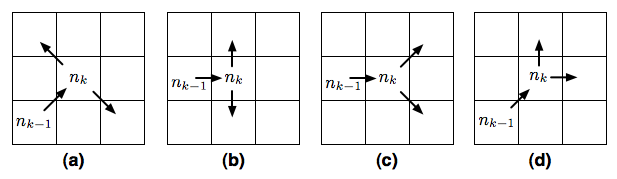
\includegraphics[width=0.95\columnwidth, trim = 10mm 10mm 10mm 0mm]
			{diagrams/turningpoints.png}
       \end{center}
	\vspace{-3pt}
       \caption{Types of optimal turning points. (a) Diagonal-to-Diagonal
(b) Straight-to-Diagonal (c) Diagonal-to-Straight.}
       \label{fig:turningpoints}
\end{figure}

\begin{theorem}
\label{theorem:jumping}
Searching with jump point pruning always returns an optimal solution. 
\end{theorem}
\begin{proof}
Let $\pi$ be an arbitrarily chosen optimal path between two nodes
on a grid and $\pi'$ a diagonal-first symmetric equivalent which is derived
by applying Algorithm \ref{alg:dfirst} to $\pi$.
We will show that every turning point mentioned by $\pi'$ is expanded optimally 
when searching with jump point pruning. We argue as follows:
\par
Divide $\pi'$ into a series of adjacent segments s.t. 
$\pi' = \pi'_{0} + \pi'_{1} + \ldots + \pi'_{n} $. Each $\pi'_{i} = \begin{pth} n_{0}, n_{1},
\ldots, n_{k-1}, n_{k} \end{pth}$ is a subpath along which all moves involve
travelling in the same direction (e.g.  only ``up'' or ``down'' etc).  Notice
that with the exception of the start and goal, every node at the beginning and
end of a segment is also a turning point.
\par
Since each $\pi'_{i}$ consists only of moves in a single direction
(straight or diagonal) we can use Algorithm \ref{alg:jump} to jump from $n_{0}
\in \pi'_{i}$, the node at beginning of each segment to $n_{k} \in \pi'_{i}$, the
node at the end, without necessarily stopping to expand every node in between.
Intermediate expansions may occur but the fact that we reach $n_{k}$
optimally from $n_{0}$ is guaranteed.
It remains to show only that both $n_{0}$ and $n_{k}$ are identified as
jump points and thus necessarily expanded. 
By Lemma \ref{lemma:turningpoints} each turning point along $\pi'$ is 
also a jump point, so every turning point node must be expanded during search.
Only the start and goal remain. The start node is necessarily expanded at the
beginning of each search while the goal node is a jump point by definition.
Thus both are expanded.
\end{proof}
